\chapter{Macro state approximation to the specific heat}
\label{chap:macrostate_approx}

Often times algorithms such as Wang-Landau (see Section \ref{sec:wang_landau}) have convergence properties proportional to the cardinality of the density of states. For many systems characterized by a low degeneracy in the lowest energy levels, the particular form of the density of states at high energies is not important when calculating derivatives of the partition function. Therefore, we find it useful to approximate these higher energy states as a single macrostate. We derive a result for the error introduced by approximating a portion of the density of states $g(x)$ as a single macro state. While the results presented here are for a continuous one-dimensional density of states, the generalization to higher dimensions or discretized states is straightforward. 

\begin{comment}
It will be quite useful to define a few shorthand functions
\begin{align}
  K_A^B(f(x)) &\equiv \int_A^B f(x) e ^ {-x \beta} dx \\
  J_A^B       &\equiv \int_A^B g(x) dx
\end{align}
For brevity we drop the functional dependence on $x$ if it is clear from the description, $g(x)=g$. The normal partition function is
\begin{equation}
  \Z = K_A^B(g)
\end{equation}
%
\end{comment}

We start with the expression of the partition function, assuming the energy range is continuous and spans the interval $A$ to $B$
\begin{equation}
\Z = \int_A^B g(x) e^{-x\beta} dx
\end{equation}
%
We approximate a small portion of the larger energies as a single macrostate in the interval $B(1-\epsilon)$ to $B$. Over this interval we assume the energy is the constant value $x_E$. The most straightforward choice for $x_E$ is a weighted average over the approximated states
\begin{equation}
x_E = \frac
{ \int_{B(1-\epsilon)}^B x g(x) e^{-x\beta} dx }
{\int_{B(1-\epsilon)}^B g(x) e^{-x\beta} dx }
\end{equation}
The approximated form of the partition function becomes
\begin{align}
\Z_\epsilon &= 
\int_A^{B(1-\epsilon)} g(x) e^{-x\beta} dx + 
\int_{B(1-\epsilon)}^B g(x) e^{-x_E\beta} dx \\
&=
\label{eq:macrostate_Zepsilon}
\int_A^{B(1-\epsilon)} g(x) e^{-x\beta} dx + 
e^{-x_E\beta} \int_{B(1-\epsilon)}^B g(x) dx
\end{align}
%
From here, we can ask how accurate this approximation is. By considering small $\epsilon$ from the term $B(1-\epsilon)$, we take a Taylor expansion around $\epsilon=0$,
\begin{equation}
  \Z_\epsilon = \sum \frac{\epsilon^n}{n!}
  \brackets{ \pfrac{\Z_\epsilon}{\epsilon^n}  }
  _ {\epsilon=0}
\end{equation}
When evaluated, this has the surprising result that the first two non-constant terms are zero
\begin{equation}
  \Z_\epsilon = \Z \epsilon^0 + 0 \epsilon^1 + 0 \epsilon^2 + \Delta \epsilon^3 + O(\epsilon^4)
\end{equation}
implying that our approximation is very good indeed.\footnote{In order to take the derivatives we recall that taking the derivative over the limits of integration can be done by
\begin{align}
\pfrac{}{a} \int_{g(a)}^b f(x) dx
=&
\pfrac{}{a} \brackets{F(b) - F(g(a))} \\
=&
- \paren{ \evalat{\frac{d F(t)}{dt}}_{t=g(a)}  } \paren{\frac{d g(a)}{d a} } \\
=&
- f(g(a)) \paren{\frac{d g(a)}{d a} }
\end{align}
where $F$ is the antiderivative of $f$.}
%
The third order term is
\begin{align}
  \Delta = 
  -\frac{B^3 g(B) e^{-B \beta}\beta^2}{24}
\end{align}
%
At very high temperatures we can approximate $\Delta$ by expanding around $\beta=0$
\begin{equation}
  \lim_{\beta\rightarrow 0} \Delta =   -\frac{B^3 g(B) \beta^2}{24} + O(\beta^3)
\end{equation}
%
If we have the explicit form for the density of states such as $g(x) = e^{\gamma x}$ (typically for Ising like systems) we can compute the expansion around $\epsilon$ to many more terms
\begin{align}
\Z_\epsilon( g(x) = e^{\gamma x} ) &= \Z \\ \notag
&-
(1/24) B^3 e^{B(\gamma-\beta)}\beta^2 \epsilon^3 \\ \notag
&+
(1/48)B^4\beta^2e^{B(\gamma-\beta)}(\gamma-\beta)\epsilon^4 \\ \notag
&- 
(1/5760)B^5\beta^2e^{B(\gamma-\beta)}(-72\beta\gamma+33\beta^2+28\gamma^2)\epsilon^5+ \\ \notag
&+ 
(1/11520)B^6\beta^2e^{B(\gamma-\beta)}(45\beta^2\gamma-40\beta\gamma^2+8\gamma^3-13\beta^3)\epsilon^6
+ O(\epsilon^7)
\end{align}
%

\subsubsection{Worked Example : Gaussian DOS}

To illustrate the power of the method we show an example at various levels of approximation. We choose a density of states that is shaped like a Gaussian, \ie a high degeneracy of intermediate states and a low probability of the extreme energies. This is characteristic of the standard Ising model; roughly, an inverted parabolic shape is found when the log of the density of states is plotted against the energies of the system. The chosen Hamiltonian is linear, again in connection with the Ising model. For convenience and clarity in plotting, we shift all energies by a constant factor $\mu=6$, so that the largest accessible state has zero energy
%
\begin{align}
  \HAM(x) &= 
  \begin{cases}
    x-\mu & 0 \le x \le \mu \\
    \infty & \text{otherwise}
  \end{cases} \\
  g(x) &= \exp  \paren{ \frac{-(x-\mu)^2}{2} }
\end{align}
In Figures \ref{fig:macrostate_ex_cut_5}, \ref{fig:macrostate_ex_cut_4}, 
\ref{fig:macrostate_ex_cut_3}, \ref{fig:macrostate_ex_cut_2}, we have plotted the approximate specific heat $CV_\epsilon$ against the exact value as a function of $\beta$. The leftmost graph shows the area of the density states that was considered a single macrostate. At low values of $\epsilon$ the approximation is nearly indistinguishable from the exact curve. In Figure \ref{fig:macrostate_ex_cut_3}, $\epsilon=\frac{1}{2}$, that we have approximated half of the state space \emph{as a single macrostate} and still achieved a reasonable approximation to the specific heat. However, if $\epsilon$ is pushed to high the resulting approximations eventually break down, ultimately creating new spurious phase changes (Figure \ref{fig:macrostate_ex_cut_2}).
%
\begin{figure}[ht]
  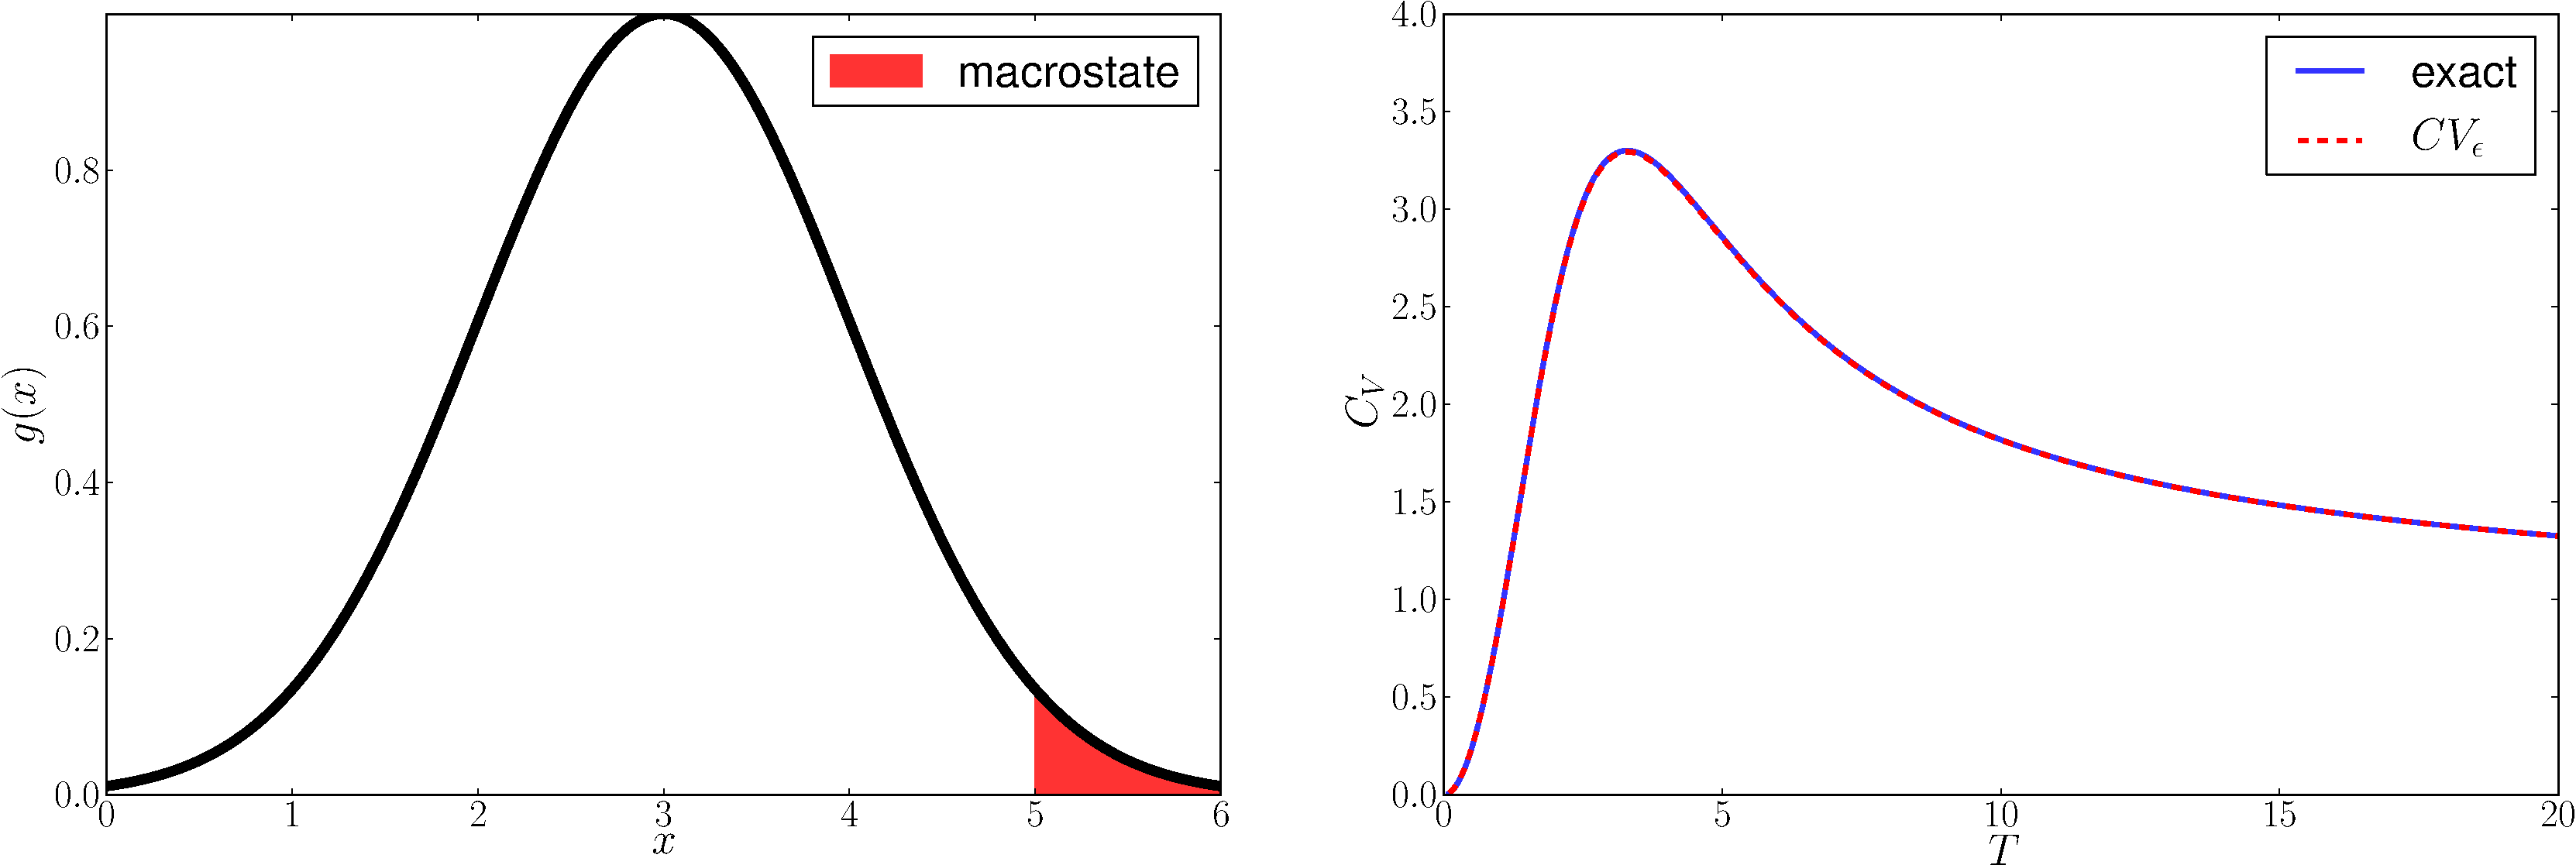
\includegraphics[width=\textwidth]{supplement/macrostate_approx_example/pictures/macrostate_epsilon_0211664312906_5.pdf}
  \caption{$CV_{\epsilon}$ with $\epsilon = 1/6$. Approximately $2.1\%$ of $g(x)$ is considered as a single macrostate (see text for details). }
  \label{fig:macrostate_ex_cut_5}
\end{figure}
%
\begin{figure}[ht]
  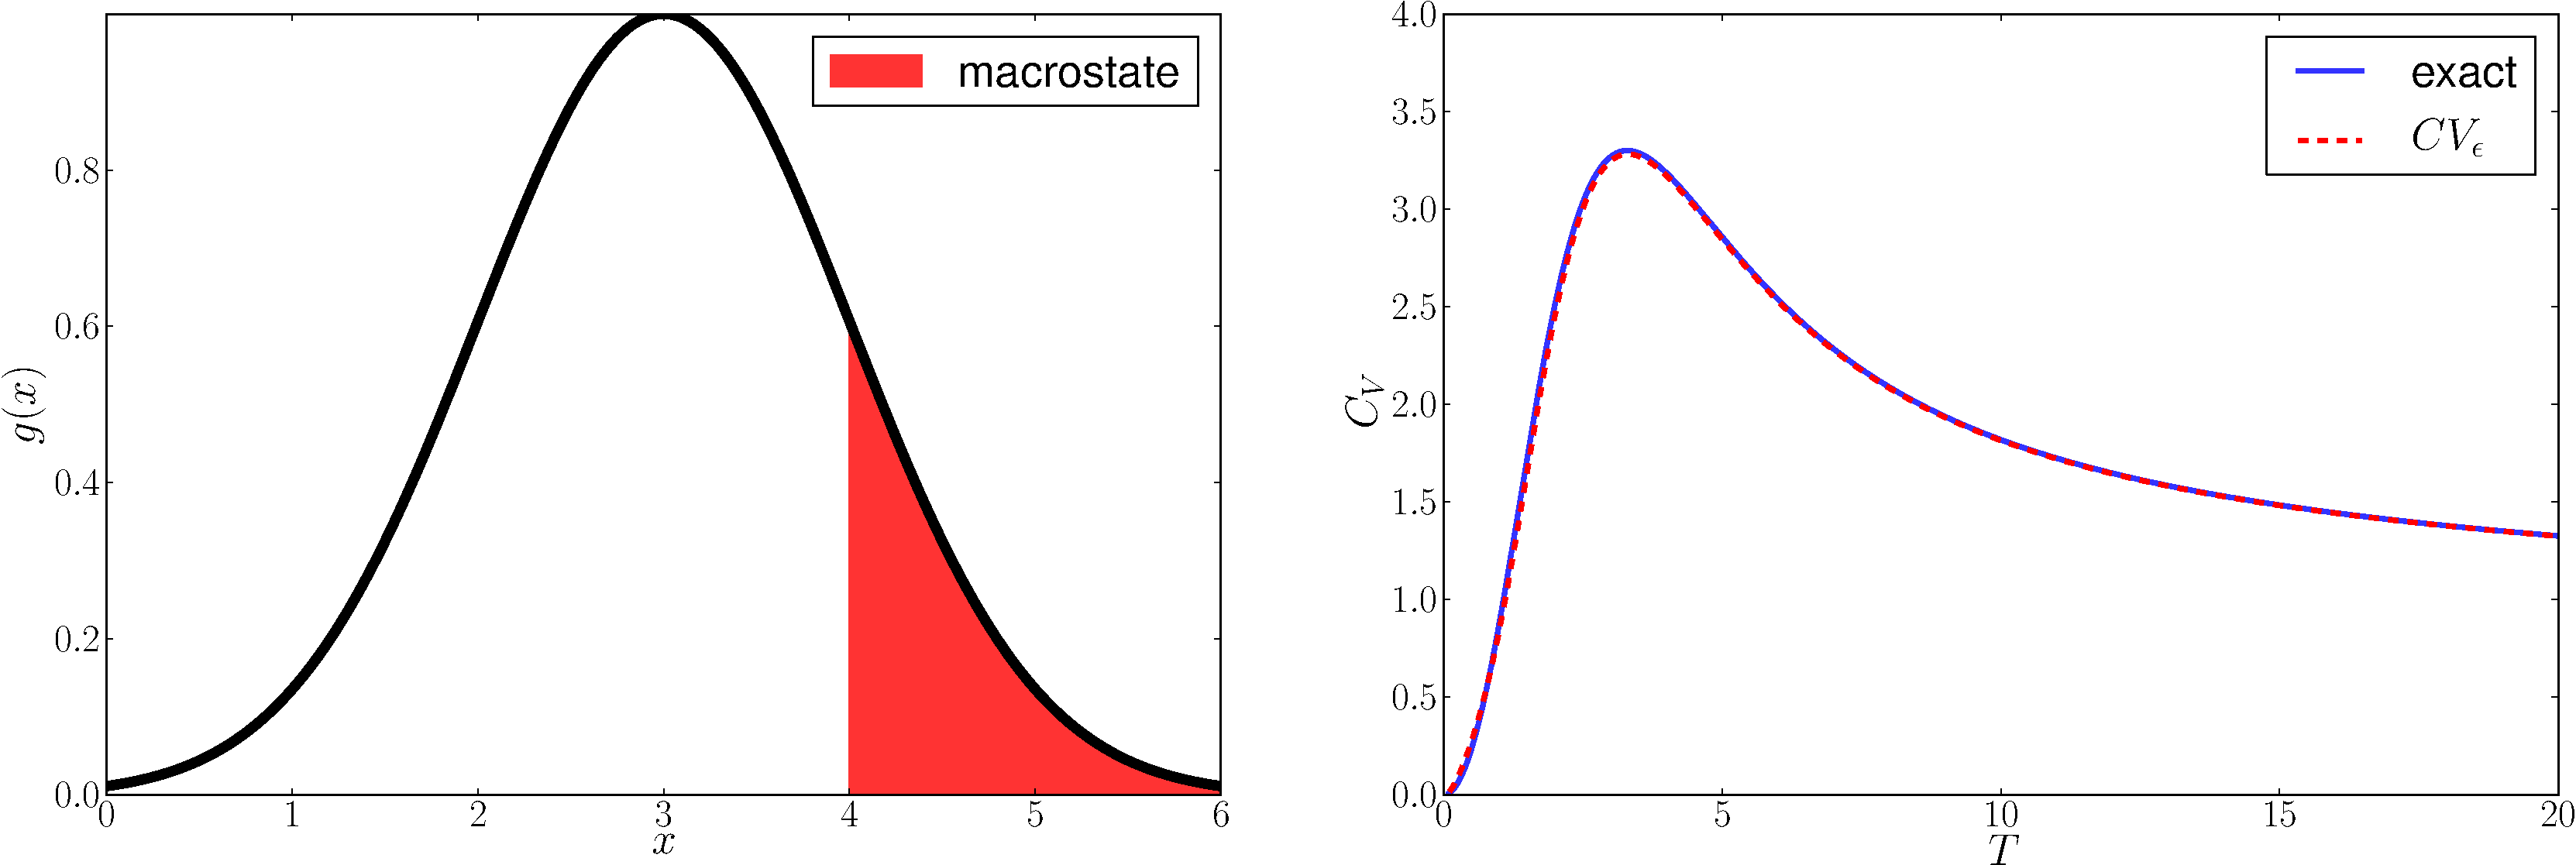
\includegraphics[width=\textwidth]{supplement/macrostate_approx_example/pictures/macrostate_epsilon_153664915749_4.pdf}
  \caption{$CV_{\epsilon}$ with $\epsilon = 1/3$. Approximately $15.7\%$ of $g(x)$ is considered as a single macrostate (see text for details). }
  \label{fig:macrostate_ex_cut_4}
\end{figure}
%
\begin{figure}[ht]
  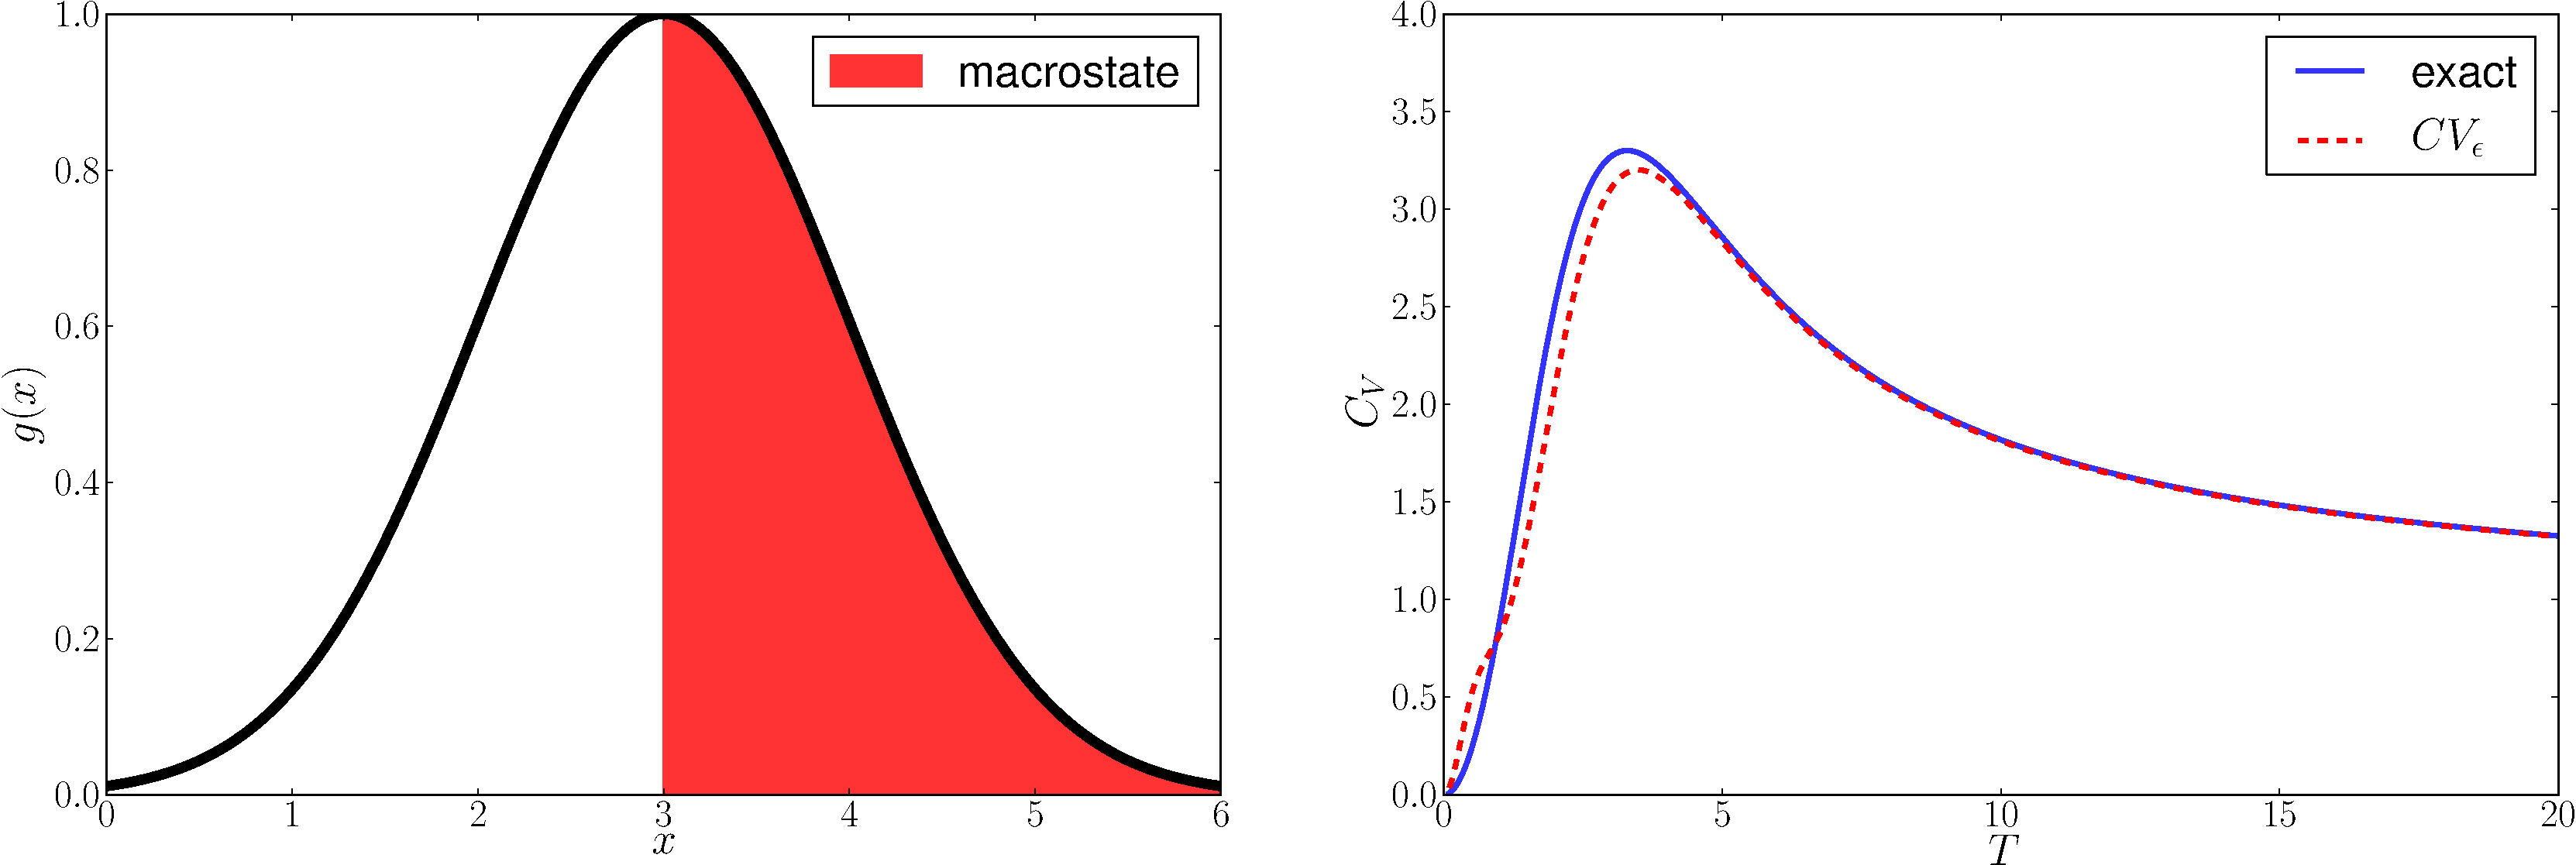
\includegraphics[width=\textwidth]{supplement/macrostate_approx_example/pictures/macrostate_epsilon_488131536823_3.pdf}
  \caption{$CV_{\epsilon}$ with $\epsilon = 1/2$. $50.0\%$ of $g(x)$ is considered as a single macrostate (see text for details). }
  \label{fig:macrostate_ex_cut_3}
\end{figure}
%
\begin{figure}[ht]
  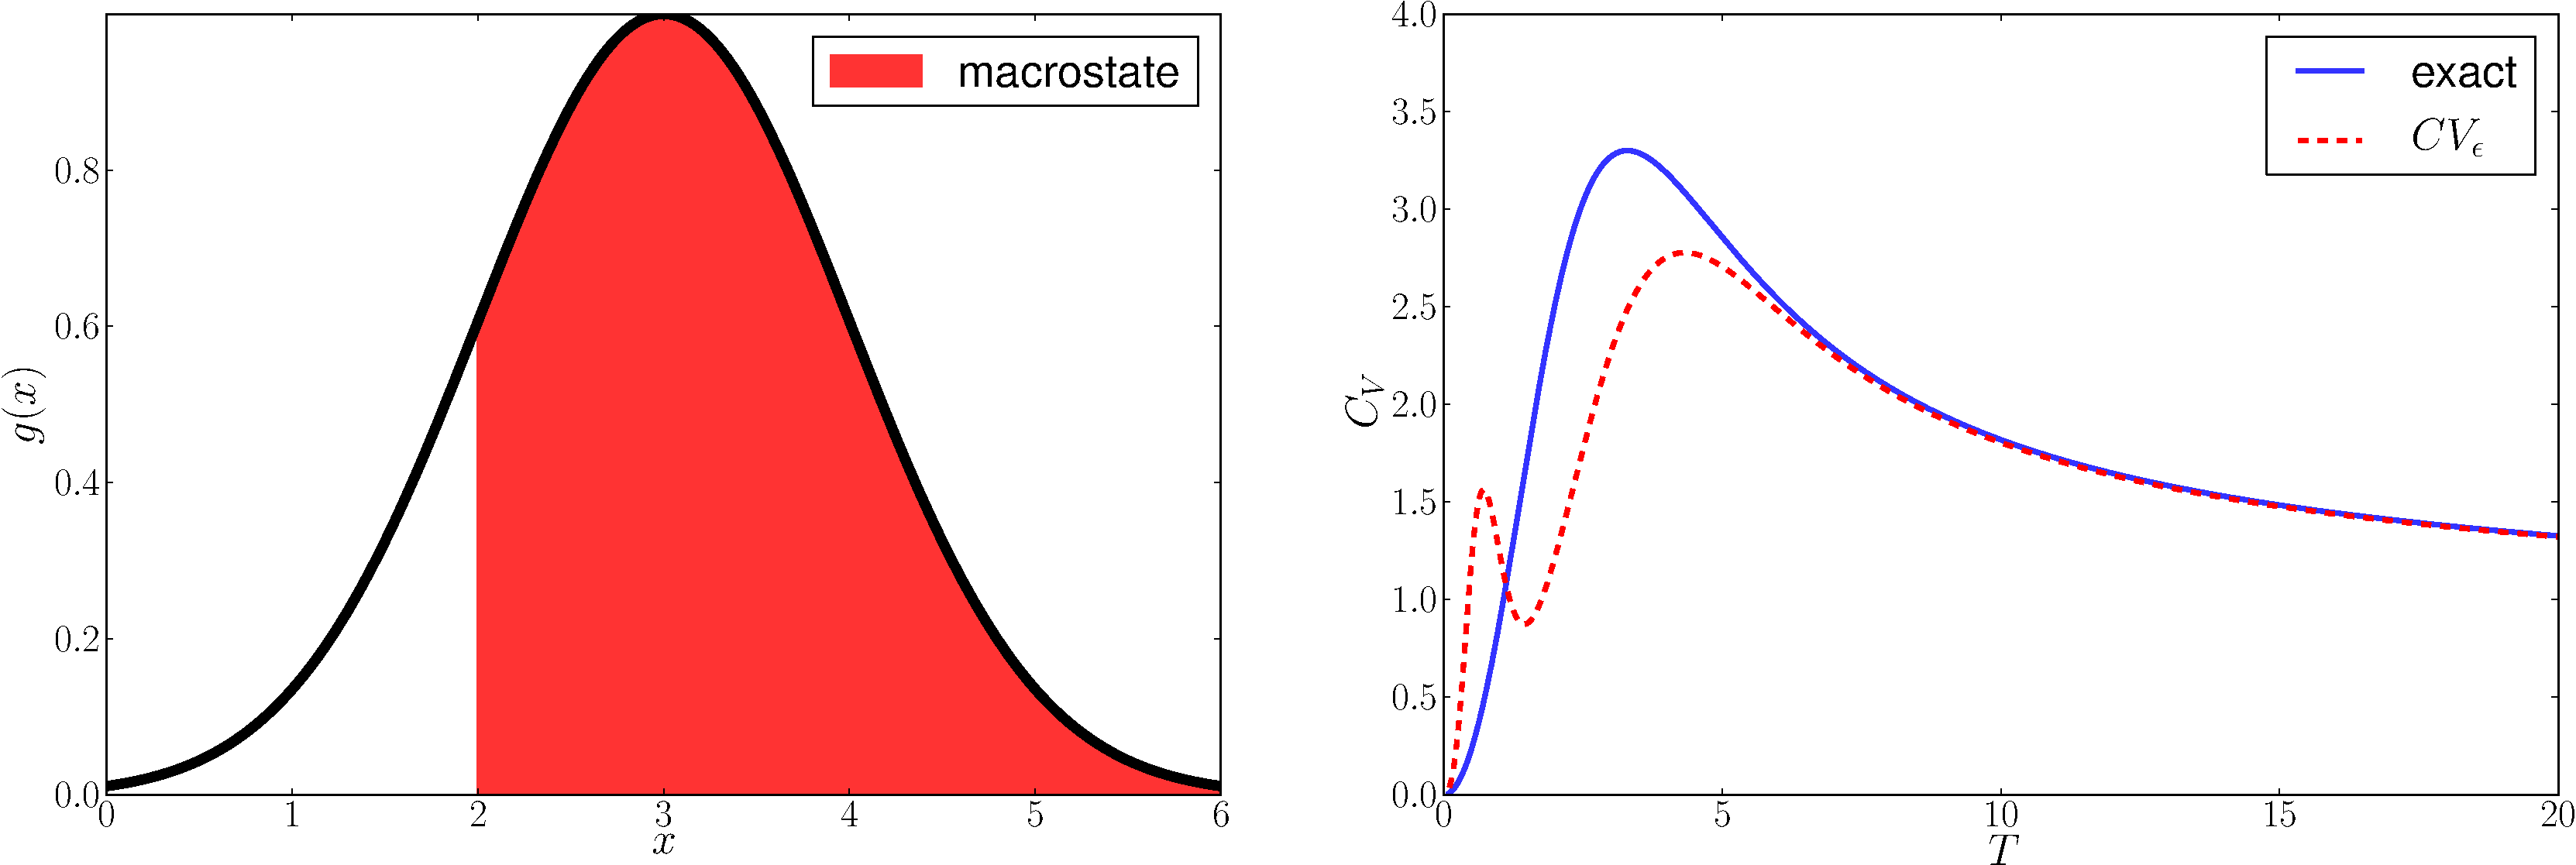
\includegraphics[width=\textwidth]{supplement/macrostate_approx_example/pictures/macrostate_epsilon_829972199084_2.pdf}
  \caption{$CV_{\epsilon}$ with $\epsilon = 2/3$. Approximately $84.2\%$ of $g(x)$ is considered as a single macrostate (see text for details). }
  \label{fig:macrostate_ex_cut_2}
\end{figure}
